\section{Problem}
	W�hrend der Entwicklung einer Software kann man immer wieder auf verschiedene Probleme treffen.
	Manche dieser Probleme betreffen die Anzeige von Daten. Hierbei sind zwei Probleme hier einmal herausgestellt:

	\begin{itemize}
		\item{Mehrere verschiedene Ansichten bei gleichen Daten.}
		\item{�nderung der Ansicht (z.B. von 2D auf 3D, Punktdiagramm, Liniendiagramm, Kreisdiagramm) bei gleichbleibenden Daten.}
	\end{itemize}

	Bei solchen oder �hnlichen Problemstellungen kann das Design Pattern MVC (Model View Controller) helfen.

\section{Definition}

	MVC behandelt drei Rollen:
	
	\begin{center}
		\fbox{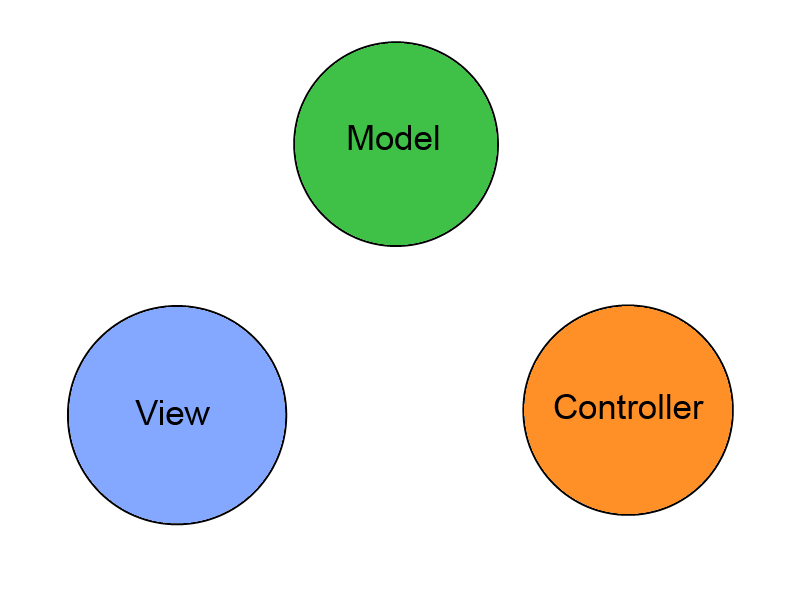
\includegraphics[scale=0.5]{figure/MVC/MVC_diagram_empty}} %low level image include -> without float
			\captionof{figure}{Model View Controller} 			%\captionof instead of \caption
		\label{pic:MVC_diagram_empty}
	\end{center}

	\subsection{Model}
		Implementiert die zentrale Struktur der Anwendung.
		Enth�lt die Gesch�ftslogik
		Schnittstelle(n) f�r Datenzugriff
		Das Model kann auch nur Proxy auf die Daten sein

	\subsection{View}
		Repr�sentiert die Anzeige des Models in dem User Interface.

	\subsection{Controller}
		Verwaltet Benutzereingaben, manipuliert das Model und aktualisiert die View\\ \\
		Es gibt keine Standarddefinition f�r MVC. Viele Frameworks benutzen unterschiedliche Versionen.\\

	\textbf{Connelly Barnes}: "'An easy way to understand MVC: 
	the model is the data, the view is the window on the screen, and the controller is the glue between the two."'\\

	\section{Schl�sselaspekte von MVC}

	\begin{itemize}
		\item{Die View/Ansicht von dem Modell trennen.}
		\item{Erm�glicht es mehrere verschiedene User Interfaces zu implementieren und die Module besser zu testen.}
		\item{Den Controller von der Pr�sentation trennen.}
		\item{Besonders n�tzlich mit Web Interfaces. (bei GUI frameworkds eher weniger)}
	\end{itemize}

	\textbf{Martin Fowler}: "'The irony ist hat almost every version of smalltalk didn't actually make a view/controller separation"'\\

\section{Unterschiedlche MVC Definitionen}
	MVC wurde von \textbf{Trygve Reenskaug} im Jahre 1979 das erste Mal beschrieben.\\

	Eine der ersten Diskussion "'A Cookbook for Using the Model-View-Controller User Interface Paradigm in Smalltalk-80"'
	 im JournalOfObjectOrientedProgramming (JOOP), von \textbf{Glenn Krasner} und \textbf{Stephen Pope}, erschien im August/September 1988.\\

	Danach wurden durch st�ndige Weiterentwicklung und Anpassung viele verschiedene Definitionen von MVC entwickelt.\\

	Die bekanntesten und wichtigsten werden hier aufgef�hrt:

	\subsection{MVC in Smalltalk '80}
	\begin{center}
		\fbox{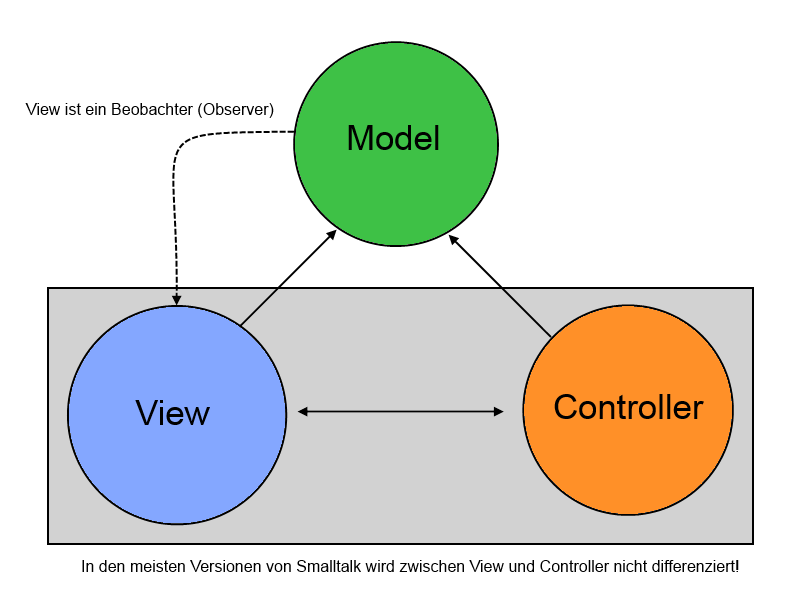
\includegraphics[scale=0.5]{figure/MVC/MVC_diagram_smalltalk}} %low level image include -> without float
			\captionof{figure}{Smalltalk Model View Controller} 			%\captionof instead of \caption
		\label{pic:MVC_diagram_smalltalk}
	\end{center}

	\subsubsection{Schl�sselaspekte}
	\begin{itemize}
		\item{Das Model ist weder von der View noch dem Controller abh�ngig.}
		\item{Bei �nderungen am Model, werden durch das \textbf{Observer Pattern} die Views aktualisiert.}
		\item{Smalltalk '80 hat View und Controller nicht getrennt.}\\
	\end{itemize}


	\begin{lstlisting} [caption={Model Klasse}\label{lst: Model_bsp},captionpos=t] 
	class ModelCounter
	    constructor: ->
	        @observers = []
	        @value = 1
	
	    increaseValue: (delta) =>
	        @value += delta
	        @notifyObservers()

	    notifyObservers: =>
	        obj.notify(this) for obj in @observers

	    registerObserver: (observer) =>
	        @observers.push(observer)
	\end{lstlisting}

	\begin{lstlisting} [caption={View/Controller Klasse}\label{lst: View_Controller_bsp},captionpos=t] 
	class ViewCounterButton
	    constructor: (opts) ->
	        @model_counter = opts.model_counter
	        @button_class = opts.button_class or 'button_counter'
	        @model_counter.registerObserver(this)

	    render: =>
	        elm = $("<button class=\"#{@button_class}\">
	                #{@model_counter.value}</button>")
	        elm.click =>
	            @model_counter.increaseValue(1)
	        return elm

	    notify: =>
	        $("button.#{@button_class}").replaceWith(=> @render())
	\end{lstlisting}